\section{Постановка задач}
Провести оптимизацию нейтральной и депротонированной форм молекулы методом B3LYP/6-31G. Расчитать полную энергию систем с учетом сольватации методом B3LYP/6-311G++(2d,p). Привести следующие результаты: 
\begin{itemize}
    \item значения полной энергии с учетом сольватации и энергию сольватации;
    \item значение $pK_a$.
\end{itemize}

\begin{figure}[H]
\centering
\captionsetup{justification=centering}
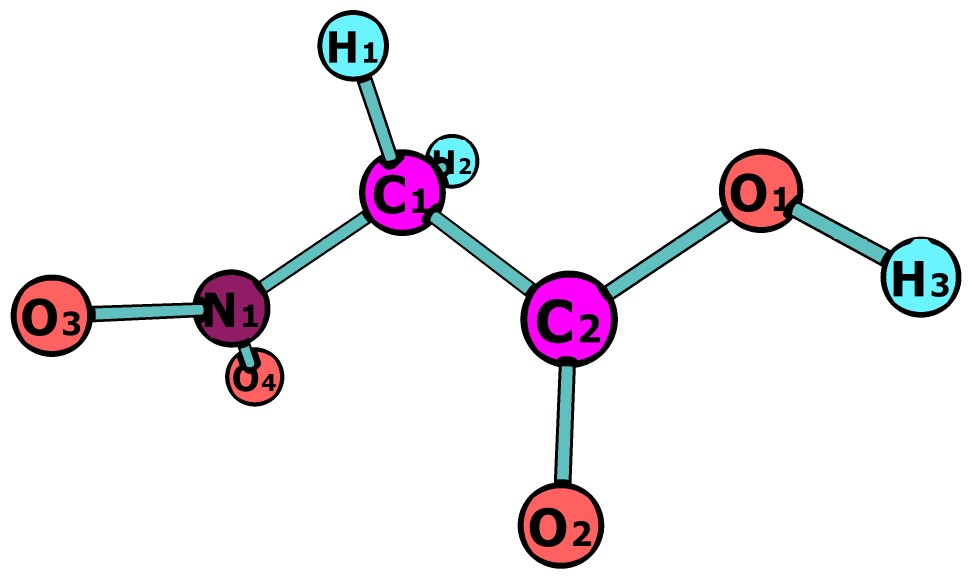
\includegraphics[scale=0.4]{fig/0.jpg}
\caption{Молекула нитроуксусной кислоты}
\end{figure}